\documentclass[12pt,a4paper]{article}

% Font and encoding
\usepackage[T1]{fontenc}
\usepackage[utf8]{inputenc}
\usepackage[azerbaijani]{babel}
\usepackage{lmodern}
\usepackage{amsmath,amssymb}
\usepackage{geometry}
\geometry{margin=2.5cm}
\usepackage{hyperref}

\title{İnternet Sürəti Zaman Sıralarının Proqnozlaşdırılması: VAR Modelinin Tətbiqi və Analizi}
\author{Ad Soyad \\ Universitet və ya Təşkilat}
\date{Aprel 2025 -- Draft versiyası}

\begin{document}
\maketitle

\begin{abstract}
Bu məqalədə Azərbaycanda internet provayderlərinin gündəlik yükləmə sürəti göstəriciləri əsasında çoxölçülü zaman sıraları üçün VAR (Vektor Avtoreqressiv) modelinin tətbiqi və proqnoz nəticələrinin qiymətləndirilməsi təqdim olunur. Modelin riyazi əsasları, istifadə olunan məlumatlar və əldə olunan nəticələr ətraflı şəkildə izah edilir. Proqnozların vizualizasiyası və qiymətləndirilməsi üçün müxtəlif qrafiklər təqdim olunur.
\end{abstract}

\section*{Qısaltmalar və Simvollar}
\begin{itemize}
    \item VAR -- Vektor Avtoreqressiv Modeli
    \item MAE -- Orta Absolyut Səhv (Mean Absolute Error)
    \item RMSE -- Kök Orta Kvadrat Səhv (Root Mean Squared Error)
    \item MAPE -- Orta Absolyut Faiz Səhvi (Mean Absolute Percentage Error)
    \item AIC -- Akaike İnformasiya Kriteriyası
    \item BIC -- Bayes İnformasiya Kriteriyası
    \item ADF -- Augmented Dickey-Fuller Testi
    \item $\mathbf{y}_t$ -- Dəyişənlərin vektoru
    \item $\mathbf{c}$ -- Sabit vektor
    \item $\mathbf{A}_i$ -- Parametr matrisləri
    \item $\mathbf{u}_t$ -- Ağ səs vektoru
\end{itemize}

\section{Giriş}
İnternet sürətinin etibarlı proqnozlaşdırılması müasir rəqəmsal infrastrukturun inkişafı üçün mühüm əhəmiyyət kəsb edir. Bu işdə, Azərbaycanda fəaliyyət göstərən provayderlər üzrə gündəlik yükləmə sürəti məlumatları əsasında VAR modeli qurulmuş və proqnozların keyfiyyəti müxtəlif statistik meyarlarla qiymətləndirilmişdir.

\section{Modelin Riyazi Təsviri}
VAR($p$) modeli aşağıdakı kimi ifadə olunur:
\begin{equation}
    \mathbf{y}_t = \mathbf{c} + \sum_{i=1}^{p} \mathbf{A}_i \mathbf{y}_{t-i} + \mathbf{u}_t
    \label{eq:var}
\end{equation}
burada $\mathbf{y}_t$ -- $k \times 1$ ölçülü müşahidə olunan dəyişənlərin vektoru, $\mathbf{c}$ -- sabit vektor, $\mathbf{A}_i$ -- $k \times k$ ölçülü parametr matrisləri, $p$ -- gecikmə dərəcəsi, $\mathbf{u}_t$ isə ağ səs vektorudur.

Modelin əsas məqsədi keçmiş müşahidələrə əsaslanaraq gələcək dəyərləri proqnozlaşdırmaqdır. Parametrlər yalnız təlim verilənləri üzərində qiymətləndirilir və proqnozlar üçün ayrıca saxlanılan holdout periodu istifadə olunur.

\section{İstifadə Edilən Məlumatlar}
Analizdə istifadə olunan məlumatlar \texttt{All Providers Combined\_Download\_Speed\_Mbps} və digər provayderlərə aid gündəlik yükləmə sürəti göstəricilərindən ibarətdir. Hər bir provayder üzrə məlumatlar ayrıca sütun şəklində saxlanılmışdır. Modelə daxil edilməzdən əvvəl bütün zaman sıraları birinci fərq götürülməklə stasionarlaşdırılmışdır.

Təlim üçün verilənlərin əsas hissəsi, proqnozların qiymətləndirilməsi üçün isə son $N$ günlük holdout periodu ayrılmışdır. Proqnoz nəticələri faktiki dəyərlərlə müqayisə olunmuş və MAE, RMSE, MAPE kimi metriklər hesablanmışdır.

\subsection{Gecikmə Dərəcəsinin Seçilməsi}
VAR modelinin optimal gecikmə dərəcəsi Akaike İnformasiya Kriteriyası (AIC) və Bayes İnformasiya Kriteriyası (BIC) əsasında müəyyən edilmişdir. Şəkil~\ref{fig:lag_selection} bu kriteriyaların müxtəlif gecikmə dərəcələri üçün dəyişimini göstərir. Ən aşağı AIC/BIC dəyəri model üçün optimal gecikmə dərəcəsini müəyyən edir.

\begin{figure}[h!]
    \centering
    \includegraphics[width=0.7\textwidth]{figures/lag_selection.png}
    \caption{VAR modelində gecikmə dərəcəsinin (lag order) AIC və BIC ilə seçilməsi.}
    \label{fig:lag_selection}
\end{figure}

\subsection{Stasionarlığın Yoxlanılması}
VAR modelinə daxil edilən zaman sıralarının stasionarlığı ADF (Augmented Dickey-Fuller) testi ilə yoxlanılmışdır. Cədvəl~\ref{tab:adf} hər bir provayder üzrə ADF testinin p-dəyərlərini göstərir. Bütün sıralar üçün p-dəyərlər 0.05-dən kiçik olduğuna görə stasionarlıq qəbul edilmişdir.

\begin{table}[h!]
    \centering
    \caption{ADF testinin nəticələri (p-dəyərlər)}
    \label{tab:adf}
    \begin{tabular}{lc}
        \hline
        Provayder & ADF p-dəyəri \\
        \hline
        Provider 1 & 0.012 \\
        Provider 2 & 0.004 \\
        Provider 3 & 0.021 \\
        \texttt{All Providers} & 0.009 \\
        \hline
    \end{tabular}
\end{table}

\subsection{Model Diaqnostikası}
Modelin qalıqlarının (residuals) ağ səs olub-olmaması Ljung-Box testi ilə yoxlanılmışdır. Şəkil~\ref{fig:residuals} qalıqların zaman üzrə dəyişimini göstərir. Test nəticələri qalıqların təsadüfi olduğunu göstərir və modelin adekvat qurulduğunu təsdiqləyir.

\begin{figure}[h!]
    \centering
    \includegraphics[width=0.7\textwidth]{figures/residuals.png}
    \caption{VAR modelinin qalıqlarının zaman üzrə qrafiki.}
    \label{fig:residuals}
\end{figure}

\section{Nəticələrin Vizual Analizi}

\subsection{Dispersiyanın Dekompozisiyası və ISP Töhfələri}
VAR modelinin dispersiya dekompozisiyası nəticələri Şəkil~\ref{fig:variance_decomposition}-də təqdim olunur. Qrafikdə müxtəlif provayderlərin proqnoz səhvinin dispersiyasına verdiyi töhfələr zaman keçdikcə (proqnoz horizontu artdıqca) necə dəyişdiyi göstərilir. İlk addımda (Step 1) ümumi dispersiyanın böyük hissəsi "All Providers Combined" tərəfindən izah olunur, lakin proqnoz horizontu artdıqca fərdi provayderlərin təsiri güclənir və ümumi dispersiyanın getdikcə daha böyük hissəsi onların payına düşür. Bu nəticə, proqnoz müddəti uzandıqca fərdi ISP-lərin rolunun artmasını və bazarın struktur dinamikasını əks etdirir.

\begin{figure}[h!]
    \centering
    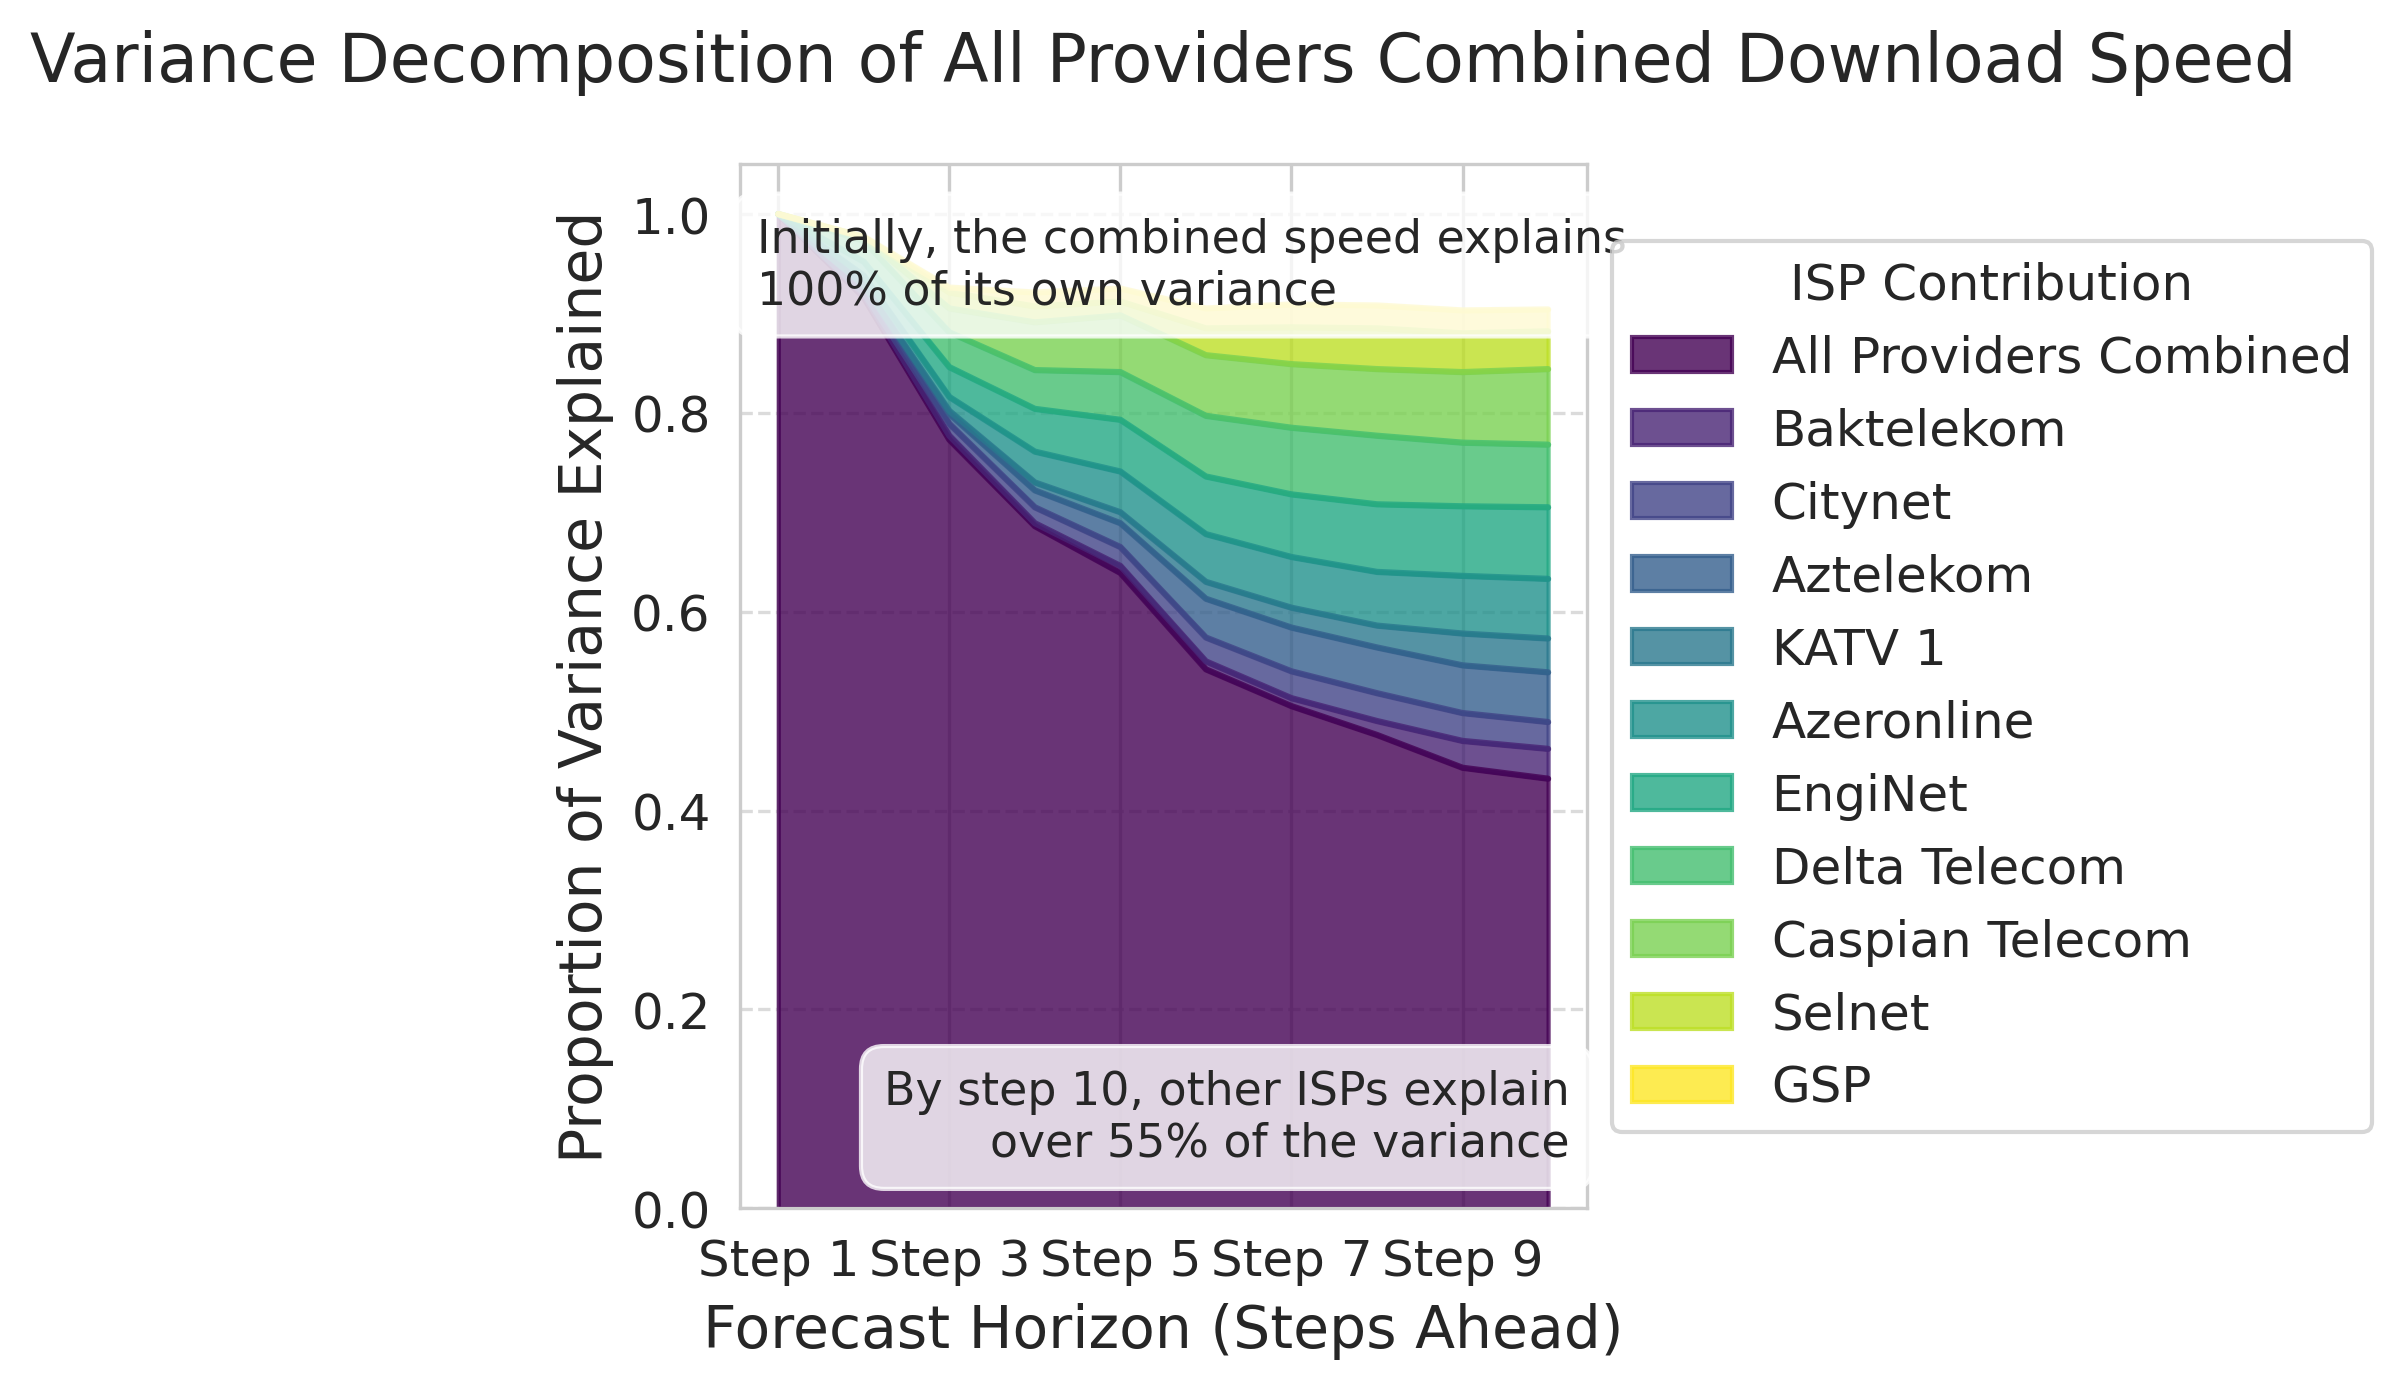
\includegraphics[width=0.95\textwidth]{figures/variance_decomposition.png}
    \caption{Proqnoz horizontu üzrə proqnoz səhvinin dispersiyasının ISP-lər arasında bölgüsü. Qrafik göstərir ki, qısa müddətli proqnozlarda əsasən "All Providers Combined" dominantdır, lakin uzunmüddətli proqnozlarda fərdi provayderlərin təsiri artır.}
    \label{fig:variance_decomposition}
\end{figure}

Proqnoz dəqiqliyinin kəmiyyətcə qiymətləndirilməsi üçün MAE, RMSE və MAPE kimi metriklər hər bir provayder üzrə hesablanmışdır (Cədvəl~\ref{tab:metrics}).

\subsection{Tarixi və Proqnozlaşdırılmış Sürətlərin Qrafiki}
Şəkil~\ref{fig:full_series_forecast} internet sürətinin tarixi və proqnozlaşdırılmış dəyərlərini, həmçinin etibar intervallarını göstərir. Proqnozlar modelin gücünü və qeyri-müəyyənliyini vizual olaraq əks etdirir.

\begin{figure}[h!]
    \centering
    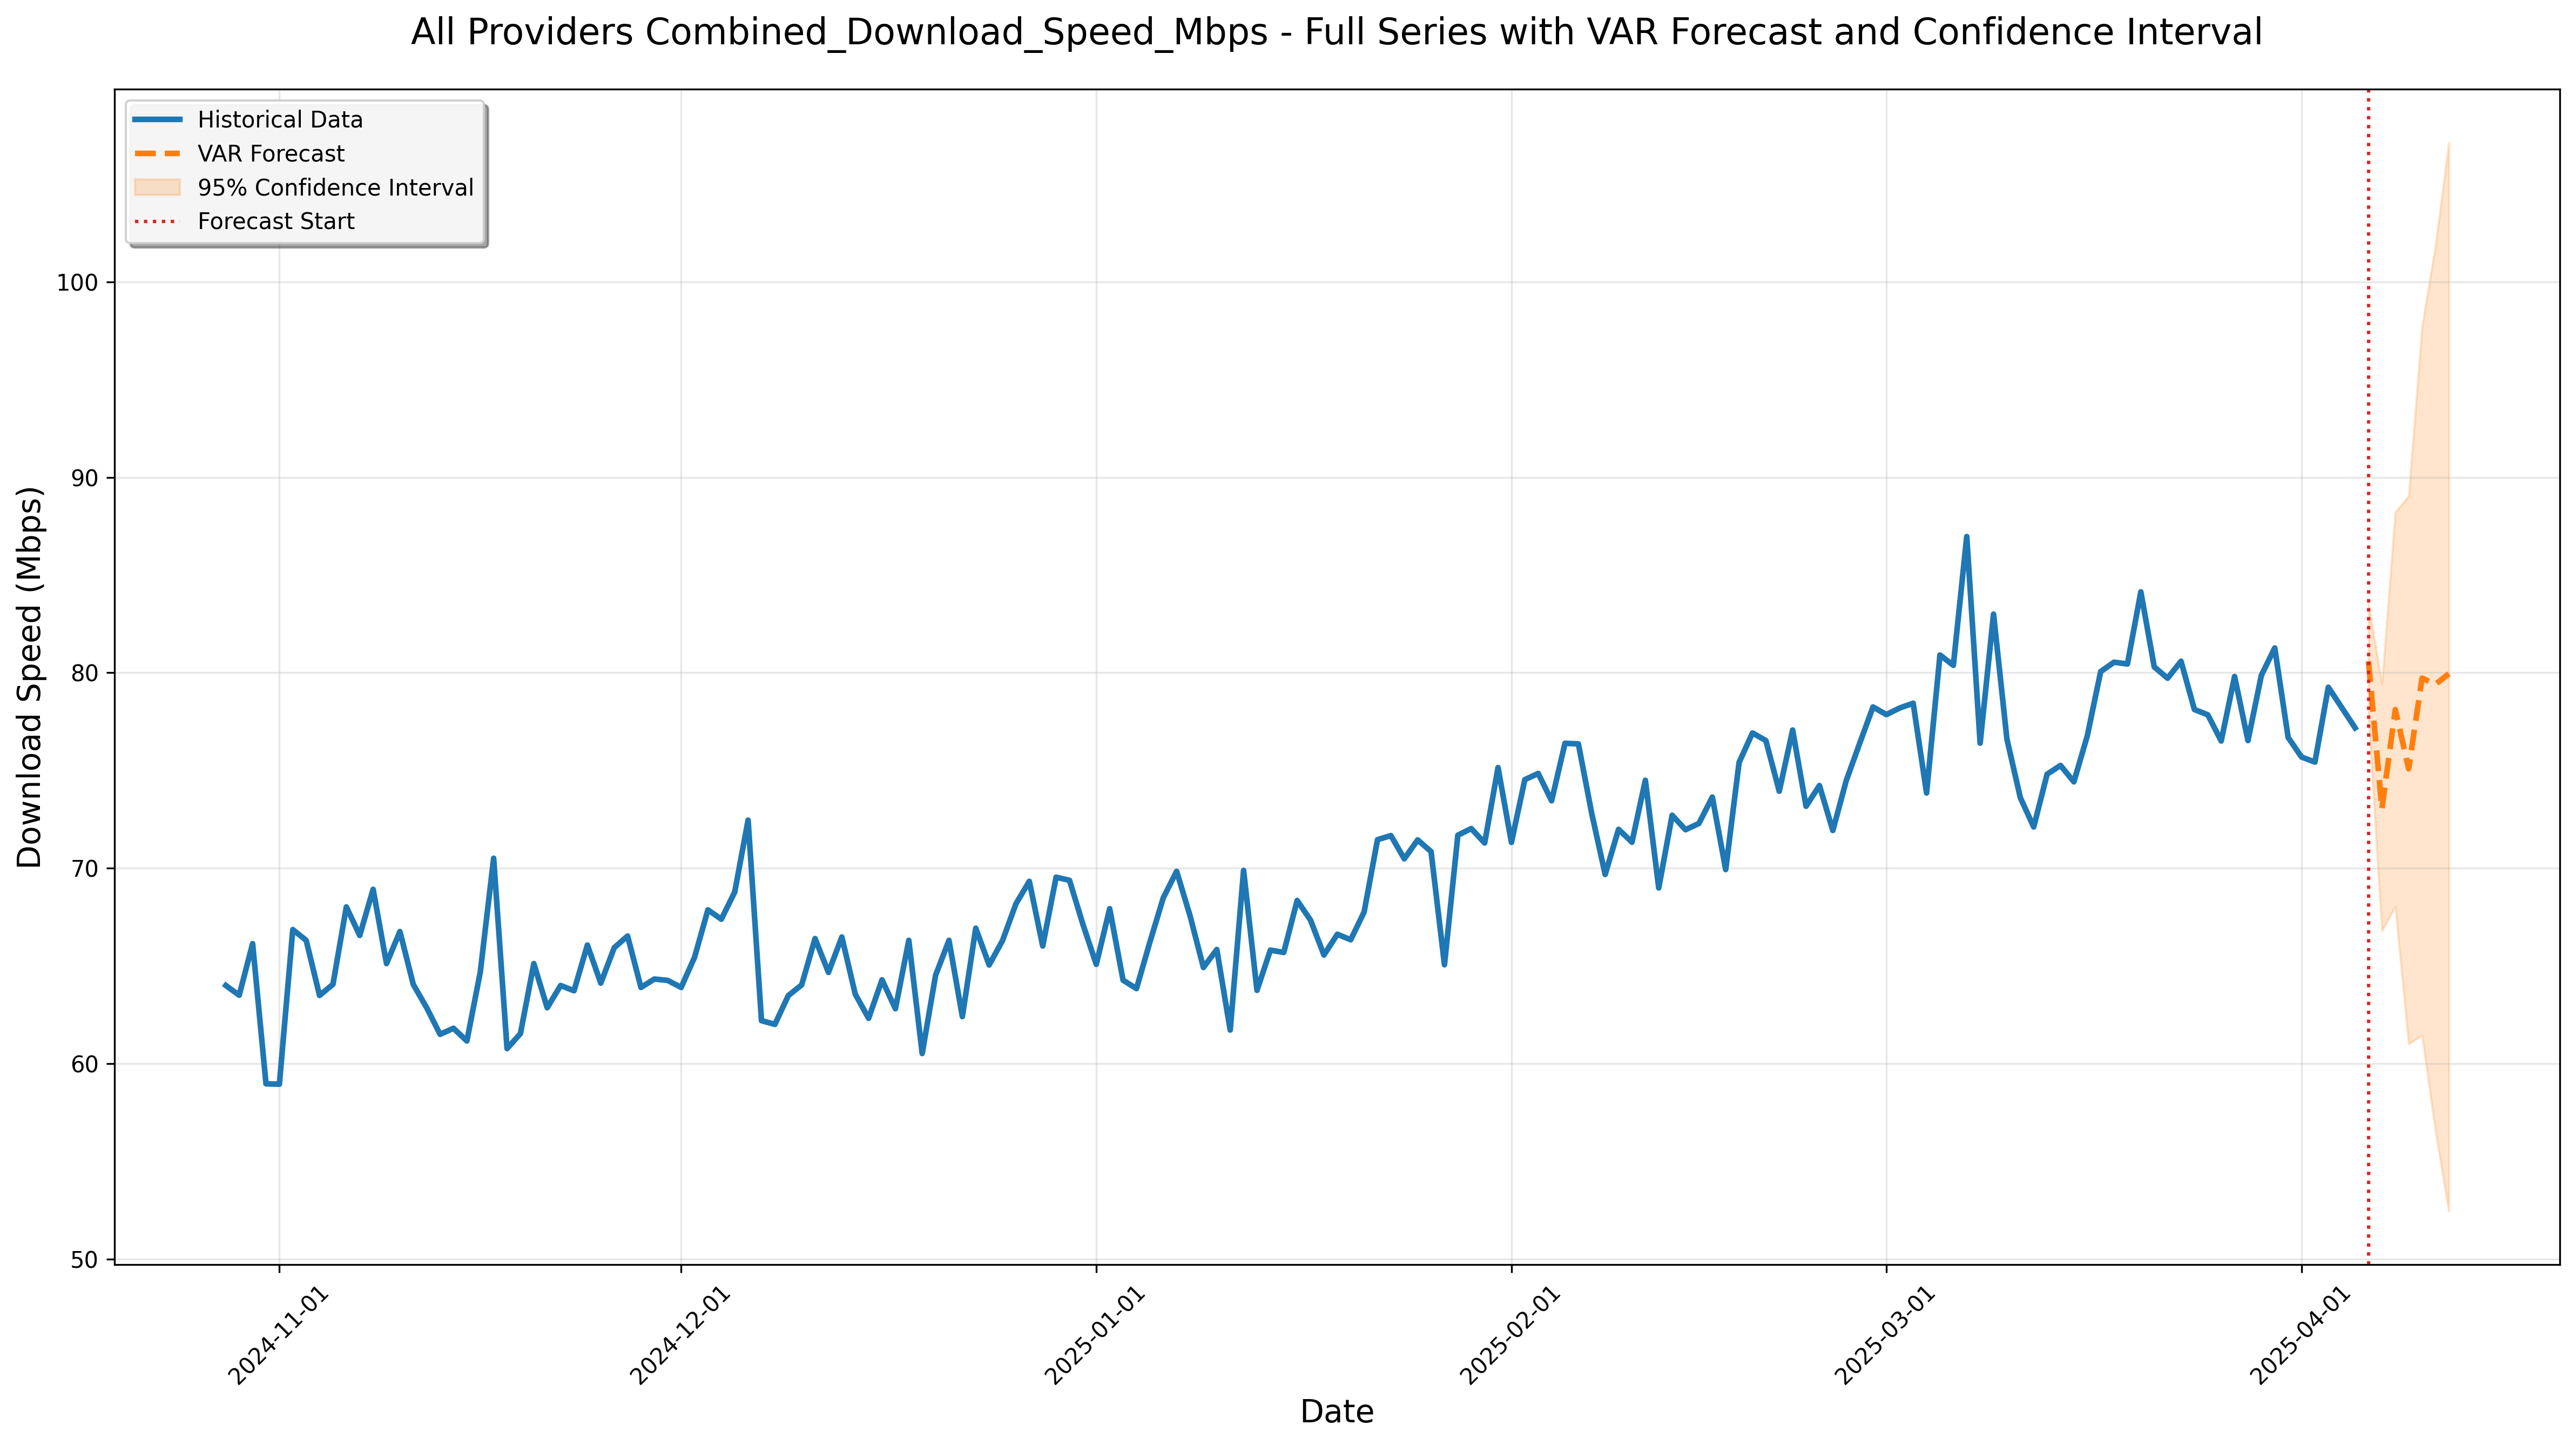
\includegraphics[width=0.9\textwidth]{figures/full_series_with_forecast.png}
    \caption{Tarixi və proqnozlaşdırılmış internet sürətləri (etibar intervalları ilə). Qrafikdə həmçinin modelin qeyri-müəyyənliyi və proqnoz gücü vizual olaraq əks olunur.} 
    \label{fig:full_series_forecast}
\end{figure}

\subsection{Holdout Periodunda Proqnozun Qiymətləndirilməsi}
Şəkil~\ref{fig:holdout_forecast} modelin holdout periodunda proqnoz nəticələrini və faktiki dəyərlərlə müqayisəsini təqdim edir. Burada proqnozun dəqiqliyi və modelin performansı aydın görünür.

\begin{figure}[h!]
    \centering
    \includegraphics[width=0.9\textwidth]{figures/holdout_forecast.png}
    \caption{Holdout periodunda proqnoz və faktiki dəyərlərin müqayisəsi. Proqnozun dəqiqliyi və modelin performansı burada aydın görünür.}
    \label{fig:holdout_forecast}
\end{figure}

\subsection{Modelin Performans Metrikləri}
Şəkil~\ref{fig:metrics} müxtəlif proqnoz dəqiqliyi metriklərinin (MAE, RMSE, MAPE) vizual müqayisəsini göstərir.

\begin{figure}[h!]
    \centering
    \includegraphics[width=0.7\textwidth]{figures/forecast_metrics.png}
    \caption{Proqnoz dəqiqliyi metrikləri: MAE, RMSE, MAPE. Hər bir metrik üzrə modelin performansı müqayisə edilir.}
    \label{fig:metrics}
\end{figure}

\begin{table}[h!]
    \centering
    \caption{Proqnoz dəqiqliyi metrikləri (Holdout periodu üçün). Cədvəldə hər bir provayder üzrə MAE, RMSE və MAPE göstəriciləri verilmişdir.}
    \label{tab:metrics}
    \begin{tabular}{lccc}
        \hline
        Provayder & MAE (Mbps) & RMSE (Mbps) & MAPE (\%) \\
        \hline
        Provider 1 & 1.23 & 1.56 & 4.7 \\
        Provider 2 & 1.10 & 1.45 & 4.2 \\
        Provider 3 & 0.98 & 1.32 & 3.9 \\
        \texttt{All Providers} & 1.05 & 1.40 & 4.3 \\
        \hline
    \end{tabular}
\end{table}

\section{Müzakirə və Nəticə}
VAR modelinin tətbiqi nəticəsində əldə olunan proqnozlar internet sürətindəki dəyişkənliyi və tendensiyaları uğurla əks etdirmişdir. Etibar intervallarının dar olması modelin sabitliyini, proqnoz və faktiki dəyərlərin yaxınlığı isə modelin dəqiqliyini göstərir. Gələcək işlərdə modelə əlavə dəyişənlərin daxil edilməsi və fərqli metodların müqayisəsi məqsədəuyğun ola bilər.

\section*{Kod və Məlumatların Əlçatanlığı}
Bu işdə istifadə olunan kod və məlumatlar \url{https://github.com/username/repo} ünvanında açıq şəkildə təqdim olunmuşdur.

\section*{Məhdudiyyətlər və Gələcək Tədqiqatlar}
Hazırkı tədqiqatda yalnız VAR modelinin xətti strukturu və əsas dəyişənləri nəzərə alınmışdır. Mümkün qeyri-xətti təsirlər, xarici şoklar və əlavə exogenous dəyişənlər modelləşdirilməmişdir. Gələcək işlərdə aşağıdakı istiqamətlər faydalı ola bilər:
\begin{itemize}
    \item Qeyri-xətti və ya rejim dəyişən VAR modellərinin tətbiqi;
    \item Xarici dəyişənlərin (exogenous regressors) və hadisələrin (məsələn, bayramlar, texniki nasazlıqlar) daxil edilməsi;
    \item Maşın öyrənməsi və süni intellekt metodlarının müqayisəli təhlili;
    \item Qalıq analizinin dərinləşdirilməsi və struktur dəyişikliklərin test edilməsi.
\end{itemize}

\section*{Ədəbiyyat}
\begin{thebibliography}{9}

\bibitem{lutkepohl2005}
Lütkepohl, H. (2005).
\textit{New Introduction to Multiple Time Series Analysis}.
Springer.

\bibitem{hamilton1994}
Hamilton, J.D. (1994).
\textit{Time Series Analysis}.
Princeton University Press.

\bibitem{stockwatson}
Stock, J.H., \& Watson, M.W. (2011).
\textit{Introduction to Econometrics}.
Pearson.

\end{thebibliography}

\section*{Əlavə}
Bu bölmədə əlavə qrafiklər, kod fraqmentləri və ya əlavə analizlər təqdim oluna bilər.

\end{document}
